
% POSTER EXAMPLE
%
% This is an example of a relatively sane poster. The box structure (and the
% narrative in general) is what I would expect, but it is completely
% non-mandatory; you may include whatever you want. Preferably, erase the
% existing box structure after you read it, and start from scratch.
%
% The main communication requirements for the poster that should be satisfied
% are as such:
%
% - At the defense, it should help you talk for around 10 minutes about your
%   thesis, and convince the committee that you did something interesting and
%   sufficiently complicated. Prepare pictures that explain your main results.
%
% - It should quickly communicate the main idea of your thesis to a random
%   educated by-walker. Ideally, a moderately-witted MFF graduate who has never
%   heard about your thesis before should be able to get the main "rough idea"
%   in less than 1 minute by just looking at the poster.

% modify the fontscale parameter to make everything slighly bigger or smaller.
\documentclass[portrait,a0paper,fontscale=0.35]{baposter}

\usepackage[utf8]{inputenc}
\usepackage[T1]{fontenc}

% FONT CHOICES
% Posters do not need to be PDF/A; you can choose any relatable font from the
% TeX font catalogue without much risk. Sans-serif fonts are suggested for the
% posters; see https://tug.org/FontCatalogue/sansseriffonts.html
\usepackage[sfdefault]{Fira Sans}
\usepackage{hyperref} 
%\usepackage[default]{droidsans}
%\usepackage[math]{iwona}
%\usepackage[defaultfam]{montserrat}
%\usepackage{cmbright}
%\usepackage{yfonts}\renewcommand{\familydefault}{\frakdefault}
\usepackage{wrapfig}
\usepackage{color}
\usepackage{graphicx}
\usepackage{multicol}
\usepackage{tasks}
\usepackage{wrapfig}
\usepackage{comment}
\usepackage{amssymb,amsmath}
\usepackage[export]{adjustbox} %allows using valign with \includegraphics

\renewcommand{\arraystretch}{1.5}

\usetikzlibrary{positioning}

% A WORD ABOUT COLORS
%
% This template is prepared with a relatively neutral gray background that
% gives decent box borders (with white and darker gray), does not clash with
% many colors (except for violet-brown and other mushroomish colors, perhaps)
% and gives a lot of space for highlighting stuff.
%
% Generally, other color variations are good too; there are no strict rules on
% the colors. Good choices include:
%
% - white backgrounds and differentiation of box headers by color (see
%   headerFontColor)
%
% - various slightly tinted backgrounds (try red!10 instead of black!3)
% 
% - dark backgrounds
%
% Keep in mind:
% - The normal "informative" text and figures should be DARK on LIGHT
%   background, not the other way around.
%
% - If you want a dark background, soften (darken) the box backgrounds a bit so
%   that they do not "shine" too much from the poster. Use \color{white} for
%   the heading, and switch the UK/MFF logos to white (see contents of logos/).
%
% - Do not mix too many color hues together. Most hues have their widely
%   accepted meaning (green: good result, red: problem, blue: information,
%   yellow: highlighter, brown: serious problem, violet: something really
%   weird/interesting/magic, depending on the shade).

\begin{document}

\color{black!80} % default font color
\begin{poster}{grid=false,
	eyecatcher=true,
	background=plain,
	bgColorOne=black!3, % background color
	columns=2,
	headerborder=none,
	textborder=none,
	headershape=rectangle,
	headershade=plain,
	boxshade=plain,
	boxColorOne=white,
	headershade=plain,
	headerColorOne=black!15, % box header background color
	headerFontColor=black,
	}%
	{
\includegraphics[height=8em]{logos/mff-black.pdf}}
	{TaleCraft — Framework for 2D\\ Point-and-Click Adventure Games}
	{\vspace{1ex} Alžbeta Kulichová | Supervisor: Mgr. Pavel Ježek, Ph.D.}
	{
\includegraphics[height=8em]{logos/uk-red.pdf}}


%
% LEFT COLUMN
%

\begin{posterbox}[column=0, span=1, name=background]{Introduction}
A typical point-and-click adventure game is a genre that emphasizes puzzle solving and often involves mystery and exploration. Players interact with in-game environments through a mouse cursor that is used to click on objects, locations, or characters in a scene to trigger actions or dialogues. Despite its seemingly straightforward gameplay, creating a point-and-click adventure game involves implementing a variety of systems, including movement, dialogue and more. 

For inexperienced developers, designing these systems can be difficult. Furthermore, there is a lack of accessible, beginner-friendly tools dedicated specifically to this genre in Unity Asset Store. To fill this demand, the goal of this thesis is to design and implement an accessible framework tailored to the development of 2D point-and-click adventure games in Unity. This framework, called \textit{TaleCraft}, will prioritize functionality and user-friendliness to help developers create games without need for advanced programming skills. This will be achieved by creating an editor in the Unity Engine that allows developers to create their desired game instead of making them write code themselves.
\end{posterbox}

\begin{posterbox}[column=0, span=1, name=goals, below=background, headerColorOne=cyan!40, boxColorOne=cyan!10]{Goals}
For this thesis we aim to meet these two goals:
\begin{itemize}
\setlength\itemsep{0.05em}
\item \textbf{Framework}. Implement a framework in Unity.
\item \textbf{Demo games.} Create two demo games to showcase the usability of our framework.
\end{itemize}

\end{posterbox}

\begin{posterbox}[column=0, span=1, name=architecture, below=goals]{Framework Design}

\begin{comment}
\begin{wrapfigure}{R}{0.4\textwidth}
\centering
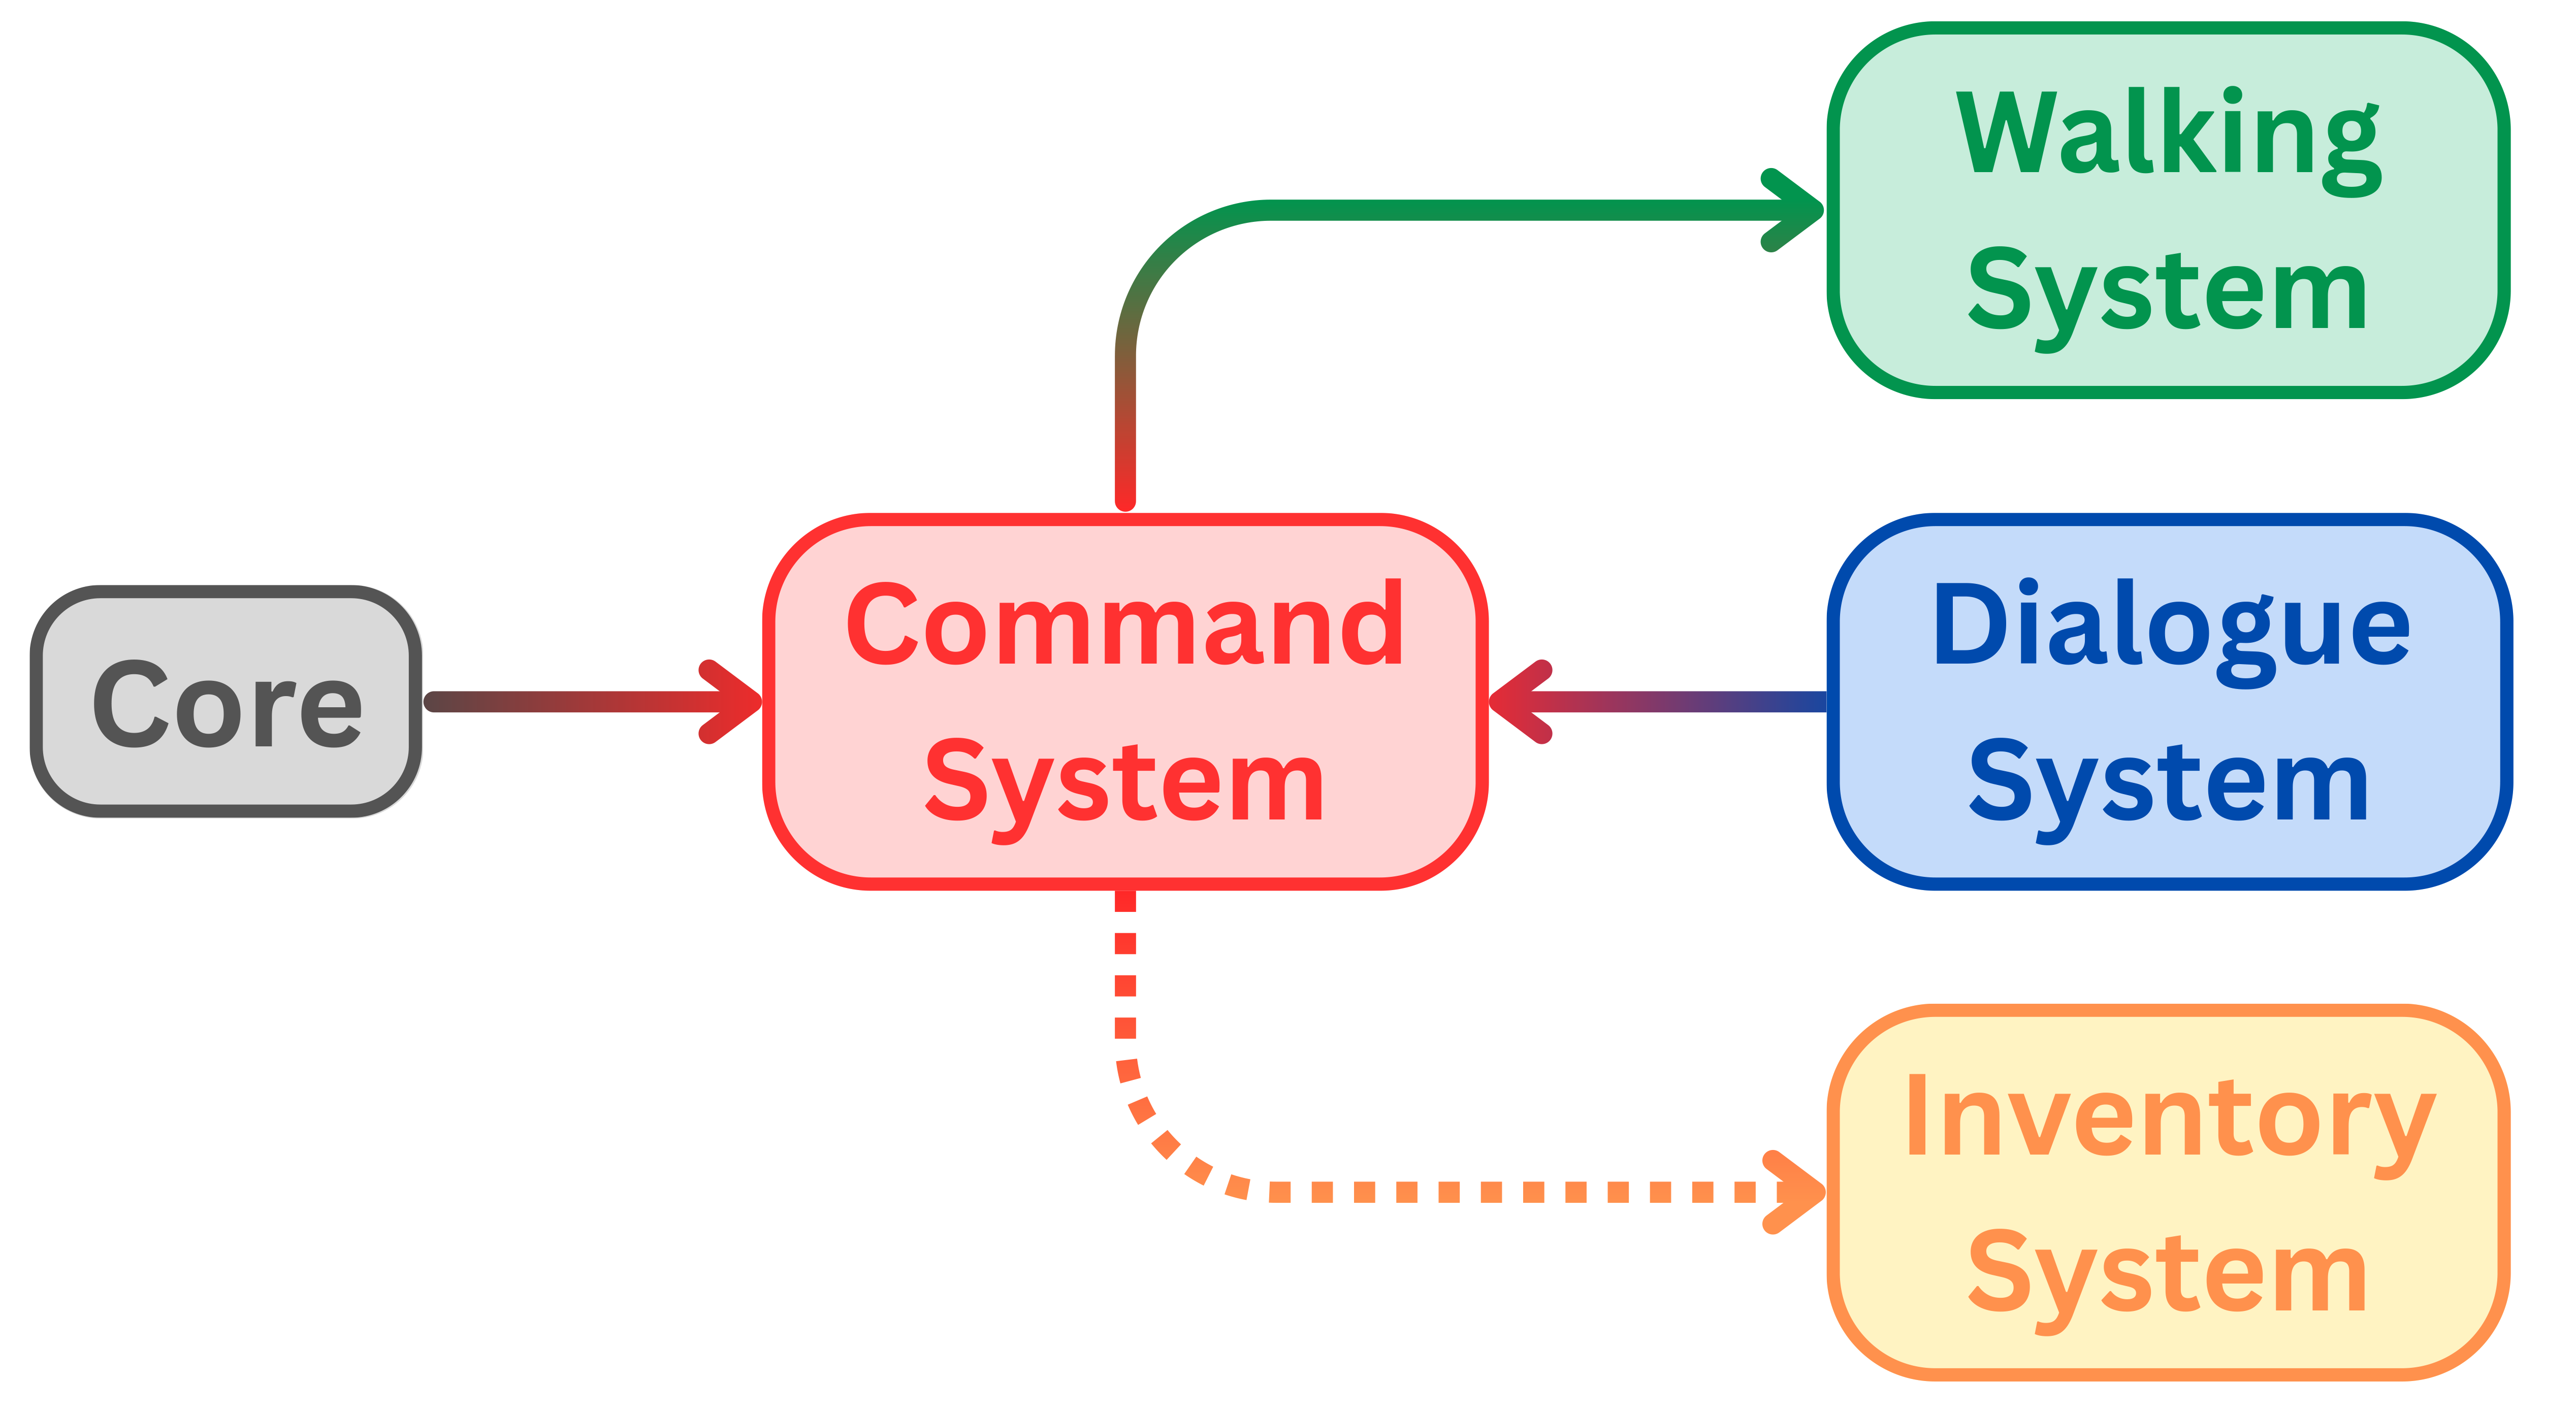
\includegraphics[width=0.35\textwidth]{img/framework.png}
\end{wrapfigure}
\end{comment}

The first goal of our thesis was to design the framework. To do this, we analyzed other games,
namely \textit{Beneath a Steel Sky}, \textit{The Secret of Monkey Island} and \textit{Fran Bow}. We then identified their common features, and divided them into the following systems:
\begin{itemize}
\setlength\itemsep{0.05em}
    \item \textbf{Commands} - Logic behind player's interactions
    \item \textbf{Movement} - Exploration of the environment by walking around
    \item \textbf{Inventory} - Storing, examining, and later using items
    \item \textbf{Dialogue} - Conversations between characters
\end{itemize}

\begin{comment}
\begin{center}
\end{center}
\end{comment}
\end{posterbox}

\begin{posterbox}[column=0, span=1, name=cs, below=architecture]{Command System}

\begin{wrapfigure}{R}{0.5\textwidth}
\centering
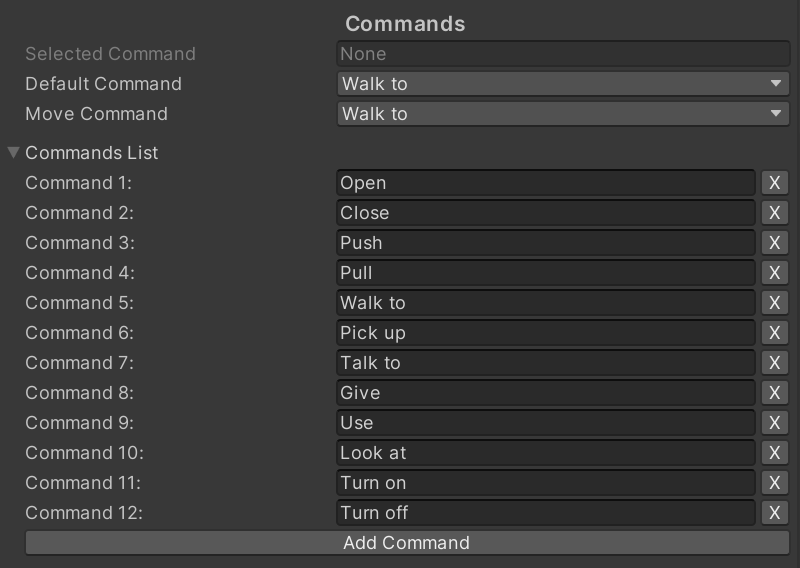
\includegraphics[width=0.48\textwidth]{img/image_2025-07-04_190803886.png}
\end{wrapfigure}

In our framework, commands represent the actions that the player wants to perform. These can be thought of as verbs, similar to those used in classic adventure games, such as \texttt{Talk to} or \texttt{Give}. We implemented a system that allows the user to define any number of commands. For example, the image on the right shows a variety of different commands that can be created. The game designer can define the logic behind each command by setting up conditions. When these conditions are met, the corresponding actions are triggered. Commands are not limited to background logic. If needed, they can also be displayed on the screen and made selectable by the player. The system additionally supports features like displaying a sentence that reflects the action the player is about to take.

\end{posterbox}

\begin{posterbox}[column=0, span=1, name=ws, below=cs]{Walking System}
In typical point-and-click games, the player is able to move around the walkable area, and TaleCraft fully supports this functionality. Walkable regions are defined using polygons. At least one polygon is required to represent the area where characters can move, while additional optional polygons can be added to represent obstacles that characters must avoid. The image below illustrates such a setup: the blue polygon defines the main walkable area, while the grey and yellow ones represent obstacles. The pink line shows a calculated path from the character's starting position to a target point. Additionally, the system supports automatic character scaling in the editor based on their position, which helps create the illusion of depth. 

\begin{center}
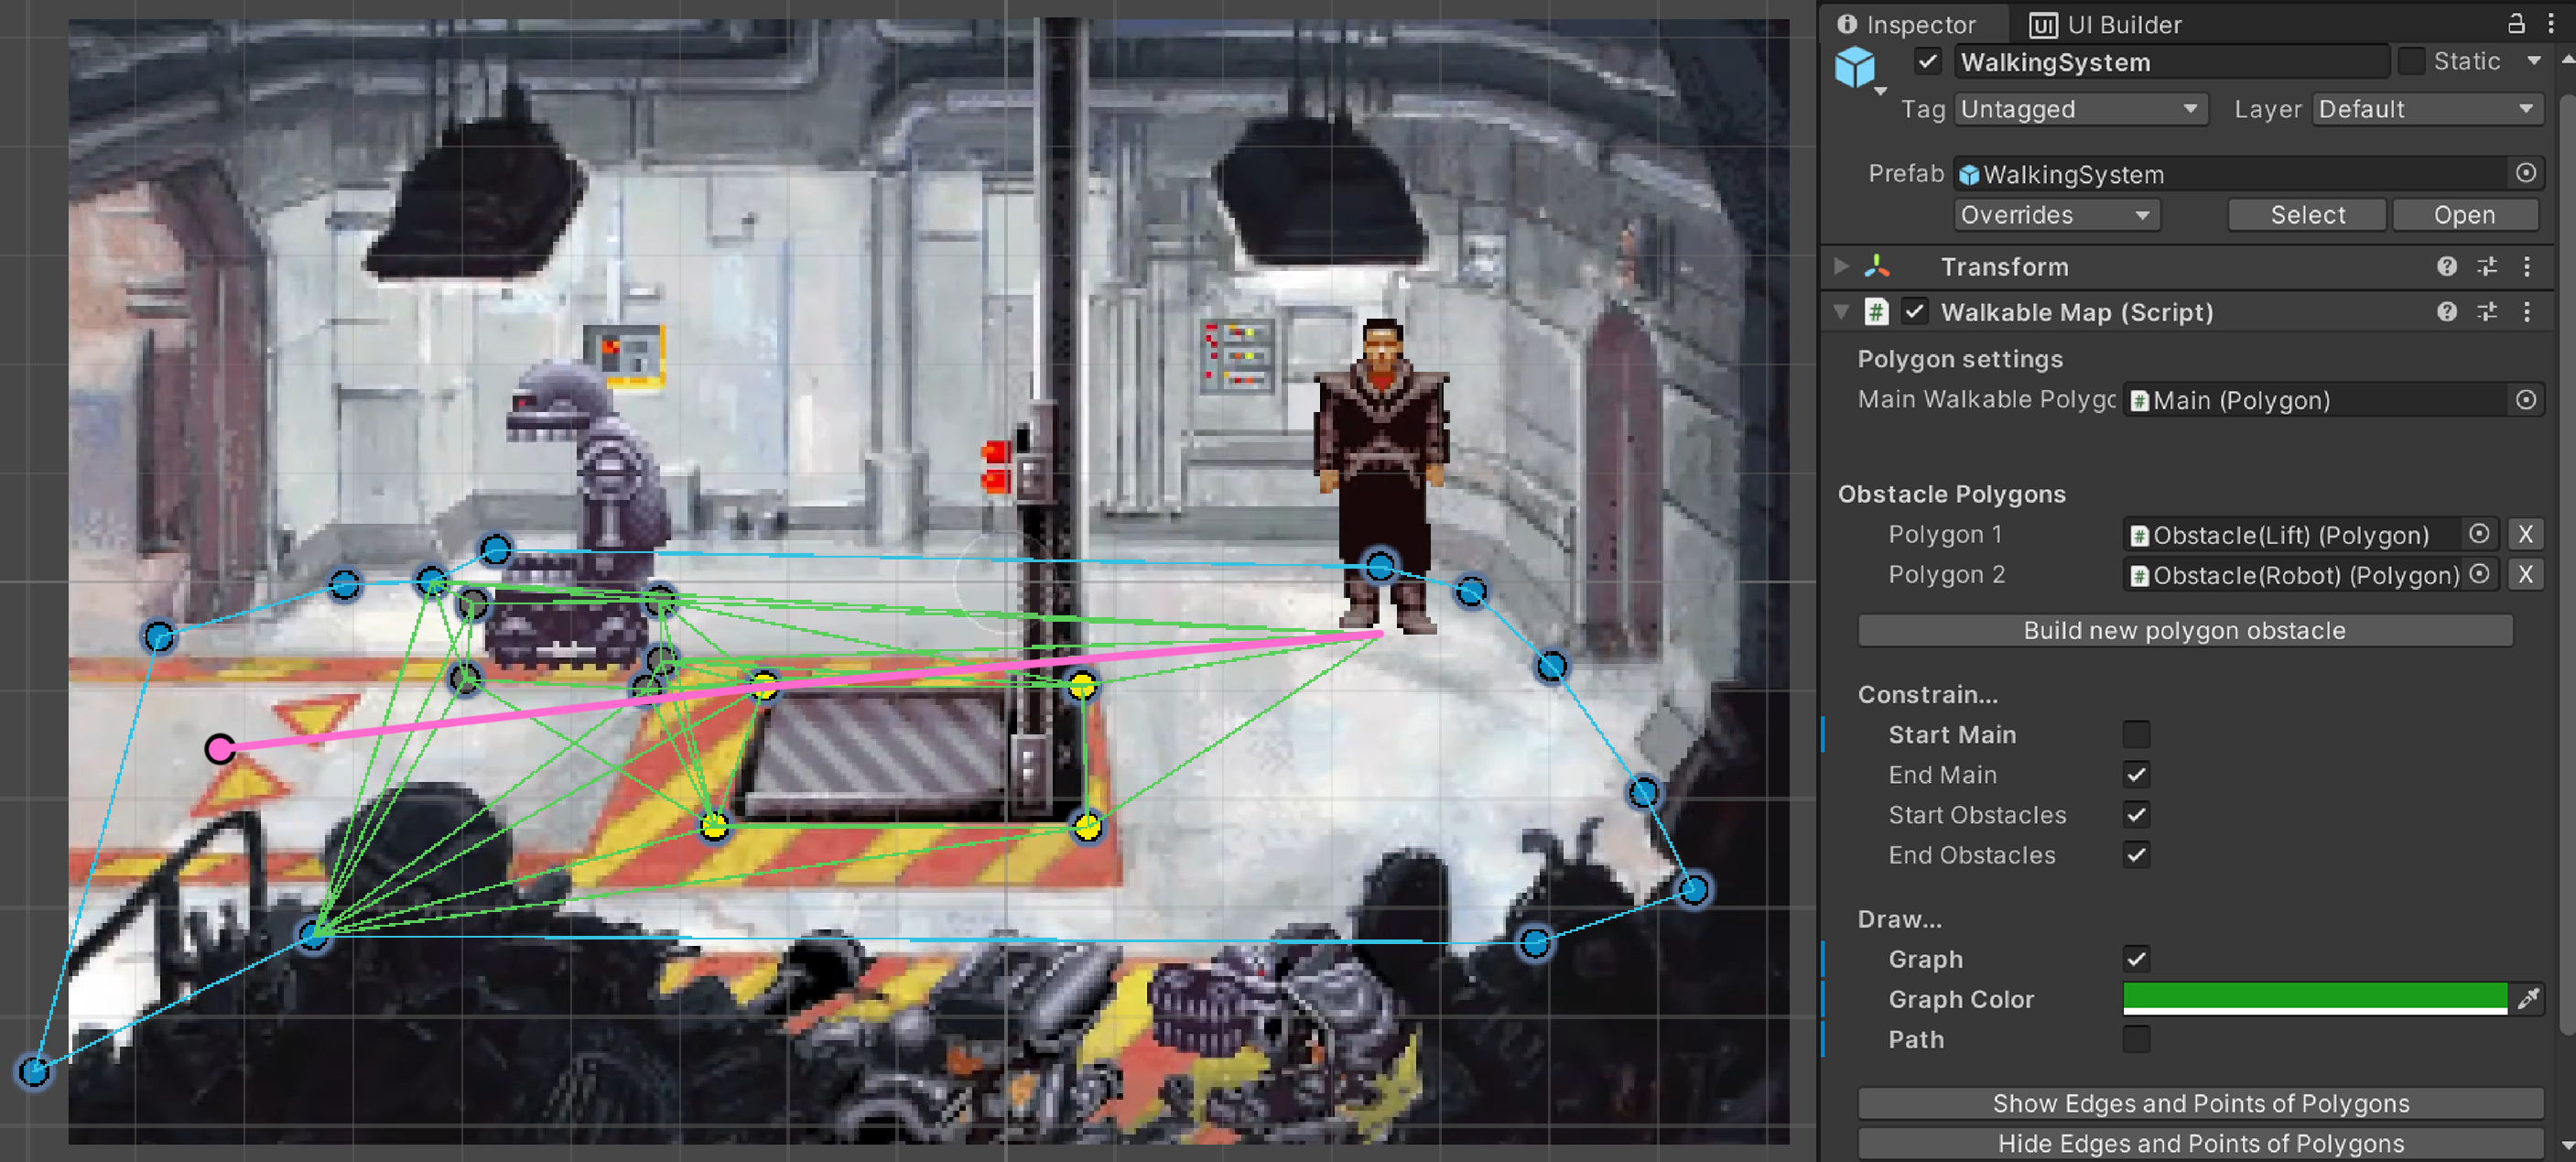
\includegraphics[width=1\linewidth]{img/walkable_map4.png}
\end{center}
\end{posterbox}

%
% RIGHT COLUMN
%
% It is usually best to fill most of the poster with your results and
% conclusions. Again, use simple annotated pictures wherever possible. Plots
% with measurements are perfect, tables are also good.
%

\begin{posterbox}[column=1, span=1, name=is]{Inventory}
To let the player collect and use items, the framework includes an inventory system. A key feature is the ability to reference inventory items across different scenes. In TaleCraft, these items are \verb|ScriptableObject|s, which makes it easy to create new items in the project and ensures they can be accessed globally. These objects store essential data such as the item's name and description, which can be used for features like displaying tags when the player hovers over an item with the mouse cursor.
\end{posterbox}

\begin{posterbox}[column=1, span=1, name=ds, below=is, %bottomaligned=info
]{Dialogue}
TaleCraft uses graphs for representing graphs, as they are ideal when dealing with complex branching conversations. They also make it straightforward to implement cyclic paths, allowing characters to revisit or repeat parts of a conversation. For TaleCraft, we defined several types of nodes that are used to construct graphs of the dialogue system.

\begin{multicols}{2}
\begin{enumerate}
\setlength
\itemsep{0.0em}
    \item \textbf{Start} - graph's starting node
    \item \textbf{Event} - executes events
    \item \textbf{Branch} - offers two ways the dialogue can progress based on criteria
    \item \textbf{Dialogue} - displays text
    \item \textbf{Choice} - displays choices
    \item \textbf{End} - graph's ending node
\end{enumerate}
\end{multicols}

\begin{center}
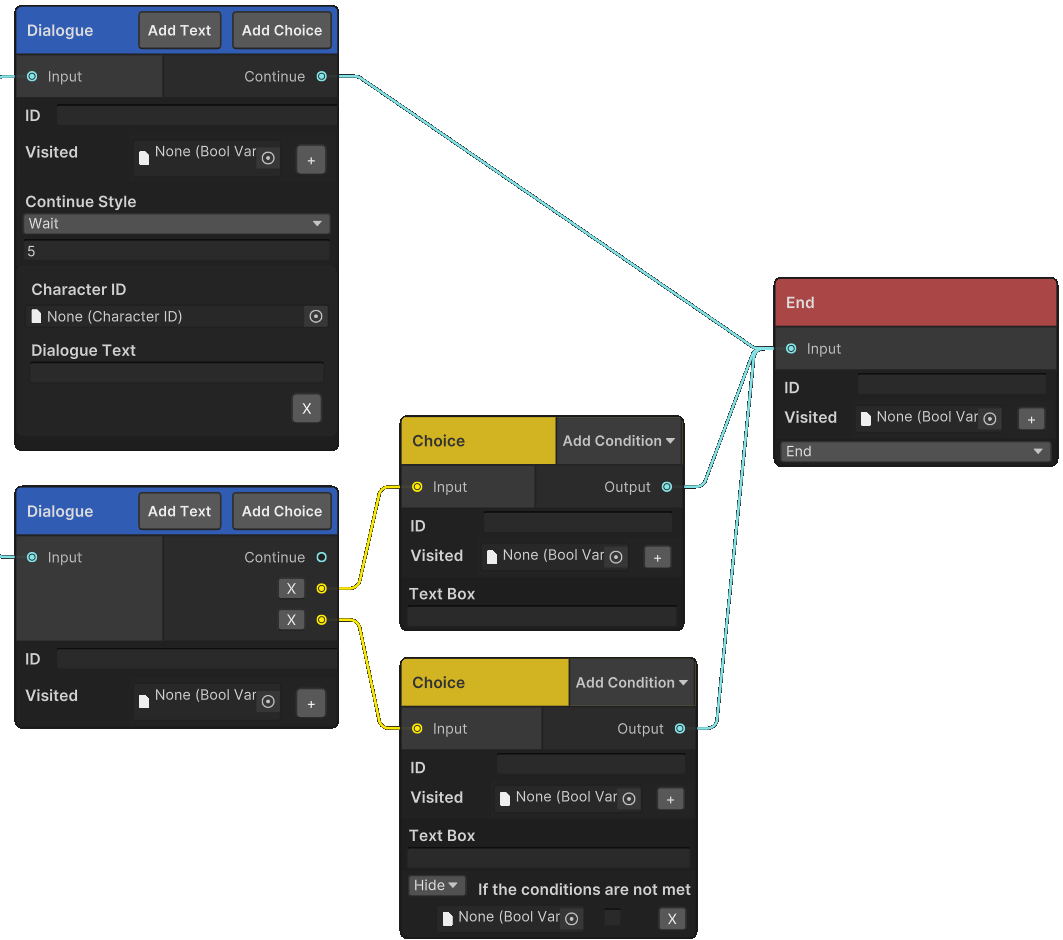
\includegraphics[width=0.7\linewidth]{img/nodes2.png}
\end{center}

%{\footnotesize
%\begin{tasks}[label=\textbullet](3)
%       \task Start
%        \task End
%        \task Dialogue
%        \task Choice
%        \task Event
%        \task Branch
%\end{tasks}}
\end{posterbox}


\begin{posterbox}[column=1, name=result2, below=ds]{Demo}
Two demo games have been developed to recreate scenes from iconic point-and-click adventure titles and to demonstrate the usability of the framework. The first demo is set in the opening location of \textit{Beneath a Steel Sky}. In this scene, the player can explore two rooms, examine various items, and engage in conversations with two characters. The second demo is based on \textit{The Secret of Monkey Island} and takes place on a street in the town of Melee Island. It showcases a scrolling screen and includes two groups of characters that the player can interact with and talk to in order to obtain items. 
\begin{center}
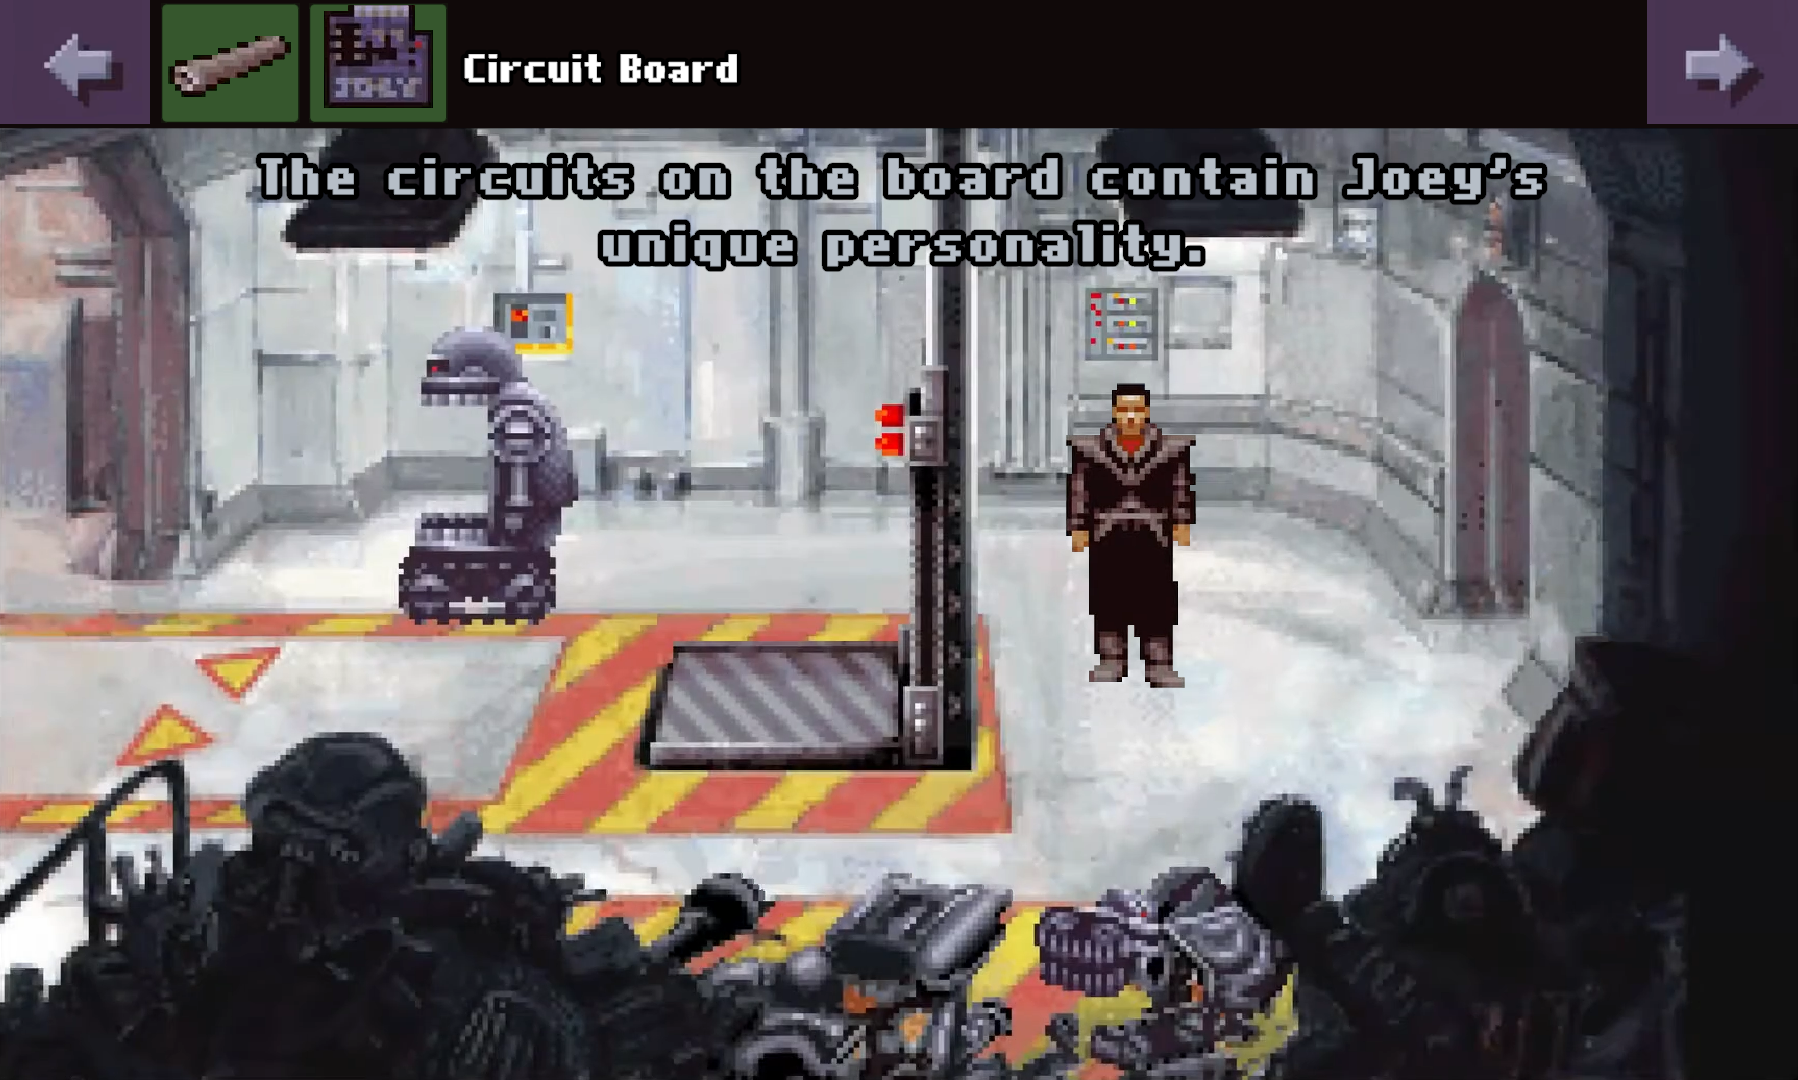
\includegraphics[width=0.506\linewidth]{img/manual.png}
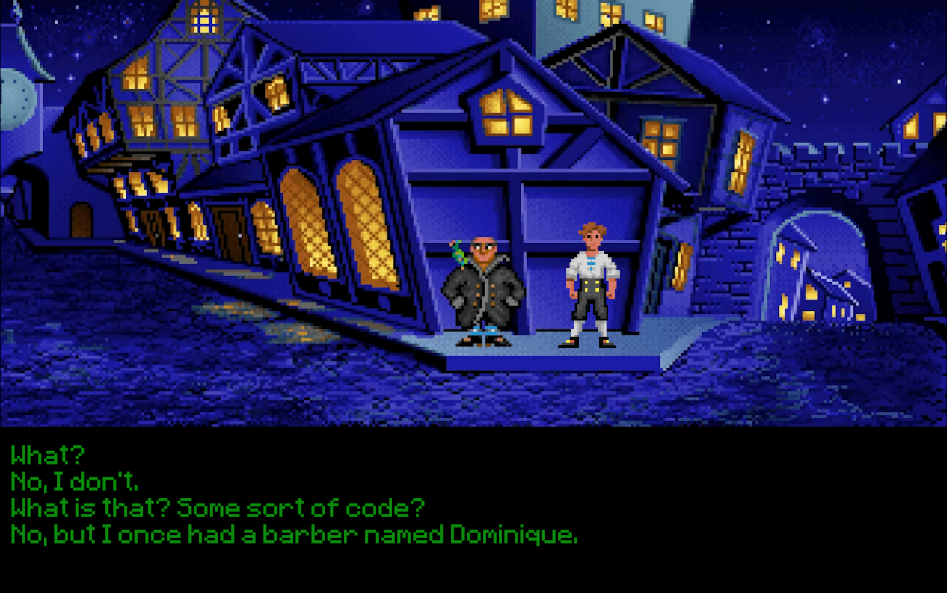
\includegraphics[width=0.486\linewidth]{img/manual-tsomi.png}
\end{center}
\end{posterbox}


\begin{posterbox}[column=1, name=conclusion, below=result2, headerColorOne=yellow!80!orange!95!black, boxColorOne=yellow!33]{Conclusion}

%\begin{wrapfigure}{r}{0.4\textwidth}
%
\includegraphics[width=1\linewidth]{img/qr.png} 
%\end{wrapfigure}

The resulting framework delivers on its objectives and serves as a foundation for developing 2D point-and-click adventure games. In addition, two simple demo games that demonstrate the capabilities of our framework have been developed. Suggestions for future work include the implementation of features that should eventually be part of the framework, the most important being animation, sound, and saving system. 

\end{posterbox}


\begin{posterbox}[column=1, name=info, below=conclusion]{Info}
\begin{comment}
\begin{wrapfigure}{R}{0.\textwidth}
\centering

\includegraphics[width=0.15\textwidth]{img/image_2025-08-06_200800481.png}
\end{wrapfigure}
\end{comment}
%\begin{tabular}{@{}p{0.65\linewidth} p{0.3\linewidth}@{}}
% Left column: everything in a parbox
 


\vspace{5mm}
    \textbf{Contact:} \\
    \href{mailto:kulichova.alzbeta@gmail.com}{kulichova.alzbeta@gmail.com} \\[1ex]
    \textbf{Project GitHub Page:} \\
    \href{https://github.com/bethkux/TaleCraft}{https://github.com/bethkux/TaleCraft}
    

%&
% Right column: QR image, top aligned

%\end{tabular}

%\begin{comment}
\begin{flushright}
\raisebox{10pt}[0pt][0pt]{%

\includegraphics[width=0.18\linewidth]{img/image_2025-08-06_200800481.png}%
}
\end{flushright}
%\end{comment}
\end{posterbox}




\end{poster}
\end{document}
